\documentclass[a4paper,12pt,oneside]{article}

\usepackage[utf8]{inputenc}
\usepackage[pdftex]{graphicx}
\usepackage{polski}
\usepackage{amsfonts}
\usepackage{verbatim}
\usepackage{indentfirst}
\usepackage{listings}
\usepackage[polish]{babel}
\usepackage[T1]{fontenc}
\usepackage{fancyhdr}
\usepackage{lastpage}
\pagestyle{fancy}
\renewcommand{\headrulewidth}{0pt}
\rhead{}
\lhead{}
\cfoot{str. \thepage/\pageref{LastPage}}

\begin{document}
\makeatletter
\addtocontents{toc}{\protect\thispagestyle{empty}}
\newcommand{\linia}{\rule{\linewidth}{0.4mm}}

\renewcommand{\maketitle}{\begin{titlepage}

    \vspace*{1cm}

    \begin{center}\small

    Politechnika Warszawska\\

    Wydział Elektryczny\\

    \end{center}

    \vspace*{1cm}

    \noindent\linia

    \begin{center}

      \LARGE \textsc{\@title}

         \end{center}

      \noindent\linia

    \vspace{1cm}

    \begin{flushright}

    \begin{minipage}{5cm}

    \textit{\small Autorzy:}\\

    \normalsize \textsc{\@author} \par

    \end{minipage}
         \end{flushright}
 \begin{center}
    \vspace{5cm}

     {\small Praca wykonana w~ramach przedmiotu:
     Języki i~metody programowania 2}

    \vspace*{\stretch{6}}

    \@date

    \end{center}

  \end{titlepage}%

}

\makeatother

\title{Specyfikacja funkcjonalna}

\title{SPECYFIKACJA FUNKCJONALNA\\projekt: wireworld}

\author{Anna Głowińska\newline numer indeksu: 291070\newline anna.glowinska98@gmail.com \newline \newline
Adam Czajka\newline numer indeksu: 291063 \newline czajka.adam147@gmail.com}

\maketitle
\tableofcontents
\thispagestyle{fancy}
\newpage
\section{Opis ogólny}

\subsection{Nazwa programu}

\textit{Wireworld} - automat komórkowy Wireworld Briana Silvermana zbudowany w~języku~\verb+Java+.

\subsection{Podstawowe pojęcia}

\noindent   \textbf{Komórka} - najmniejsza jednostka automatu komórkowego, która może znajdować się w~jednym z~czterech stanów (przypisujemy im odpowiednie kolory): pusta - czarna, głowa elektronu - niebieska, ogon elektronu - czerwony, przewodnik - żółty.
\\\\
\textbf{Automat komórkowy} - uporządkowany zbiór komórek, z~których każda znajduje się w~jednym z~kilku dozwolonych stanów. Komórki przylegają do siebie tworząc siatki.
\\\\
\textbf{Siatka} - dwuwymiarowy fragment płaszczyzny o~danych wymiarach, podzielony liniami tworzącymi macierz, składającą się z~pojedynczych komórek.
\\\\
\textbf{Generacja} - stan wszystkich komórek w~danej chwili, ale też czynność zmiany ich stanów.
\\\\
\textbf{Sąsiedztwo Moore'a} - graniczenie komórki z~innymi komórkami, warunkujące nowy stan tej komórki, na podstawie 8 przylegających komórek (znajdujących się: na południu, na południowym-zachodzie, na zachodzie, na północnym-zachodzie, na północy, na północnym-wschodzie, na wschodzie i~na południowym-wschodzie).

\subsection{Poruszany problem}
Zadaniem automatu komórkowego \textit{Wireworld} jest symulacja elementów elektronicznych operujących na wartościach bitowych. Symulacja toczy się na dwuwymiarowej płaszczyźnie podzielonej na kwadratowe komórki. Zgodnie z przyjętymi zasadami każda komórka ma ośmiu sąsiadów (sąsiedztwo Moore'a), czyli komórki przylegające do niej bokami i~rogami. Każda komórka może znajdować się w~jednym z~czterech stanów: pusta, głowa elektronu, ogon elektronu albo przewodnik). 
\par Stany komórek zmieniają się przy każdej generacji. Dana generacja jest używana do obliczenia następnej generacji. Po obliczeniu wszystkie komórki zmieniają swój stan dokładnie w~tym samym momencie. Stan komórki po generacji zależy tylko od otaczających ją sąsiadów i jej obecnego stanu oraz zmienia się zgodnie z ustalonymi zasadami.






\par Zestaw reguł przy tworzeniu nowej generacji (przejścia do następnego stanu) jest następujący:

\begin{itemize}
\item  komórka pusta $\rightarrow$ komórka pusta,

\item  głowa elektronu $\rightarrow$ ogon elektronu,

\item  przeprowadzenie zadanej liczby generacji,
\item  ogon elektronu $\rightarrow$ przewodnik,

\item przewodnik $\rightarrow$ głowa elektronu, ale tylko wtedy, gdy dokładnie 1 lub 2 komórki sąsiadujące są głowami elektronu.
\end{itemize}

\section{Wygląd programu}
\subsection{Wygląd GUI}

\begin{figure}[ht]
\centering
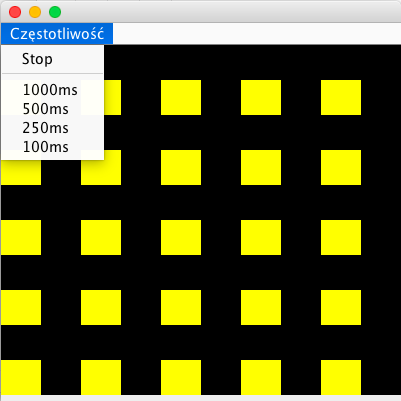
\includegraphics[width=0.65\textwidth]{gui.png}
\caption{Wygląd GUI.}
\label{fig:k1}
\end{figure}

\subsection{Opis wyglądu GUI}
Graficzny interfejs użytkownika programu \textit{Wireworld} jest reprezentowany przez okno dialogowe. Przebieg generacji odbywa się w centralnej części okna, gdzie komórki przyjmują odpowiednie kolory w zależności od ich stanu. Powyżej znajduje się pasek menu, w którym użytkownik programu dobiera częstotliwość wyświetlania kolejnych generacji oraz w wybranym  momencie zatrzymuje działanie programu i zapisuje bieżącą generację do pliku TXT.

\section{Opis funkcjonalności}


\subsection{Korzystanie z programu}
Program \textit{Wireworld} jest pisany, kompilowany oraz uruchamiany za pomocą programu \verb+IntelliJ IDEA 2017.3.5 (Community Edition)+.

\subsection{Uruchomienie programu}
Program \verb+IntelliJ+ wywoływany jest automatycznie po naciśnęciu przycisku \verb+run+.    
\subsection{Możliwości programu}

Zadania jakie wykonuje program:
\begin{itemize}
\item  wczytywanie do programu początkowej konfiguracji generacji z~pliku w~formacie TXT,
\item  wczytanie danych wejściowych z wbudowanej w program biblioteki,
\item  przeprowadzenie kolejnych generacji,
\item  wyświetlanie kolejnych generacji w czasowych odstępach o długości wybranej przez użytkownika użytkownika,
\item zatrzymanie wyświetlania kolejnych generacji,
\item  zapisywanie bieżącej generacji do pliku TXT, który może zostać potem wczytany.
\end{itemize}


\section{Format danych i~struktury plików}


\subsection{Struktura katalogów}

Szkielet projektu został przedstawiony na poniższym schemacie: \newline

\par wireworld
\par +--- data
\par \ |\ \ \ \ \  +--- data.txt
\par \ |\ \ \ \ \  +--- library
\par \ |\ \ \ \ \  +--- results
\par +--- src
\par \ |\ \ \ \ \  +--- ww
\par \ |\ \ \ \ \ \ \ \ \ \  +--- tests

\par +--- out
\par \ |\ \ \ \ \  +--- production
\par \ |\ \ \ \ \ \ \ \ \ \  +--- wireworld
\par \ |\ \ \ \ \ \ \ \ \ \ \ \ \ \ \  +--- ww
\newline

gdzie: \par \verb+wireworld+ - katalog projektu,
\par \verb+data+ - katalog zawierający dane testowe (dane.txt) oraz katalogi \verb+library+ i \verb+results+,
\par \verb+library+ - katalog zawierający przykłady danych wejściowych w plikach TXT,
\par \verb+results+ - katalog w którym zostają zapisane bieżące generacje w~formacie TXT,
\par \verb+src+ - katalog zawierający pliki z kodem programu,
\par \verb+tests+ - katalog zawierający pliki z kodem poszczególnych testów,
\par \verb+out+ - katalog zawierający pliki wykonywalne.

\subsection{Przechowywanie danych}
\textbf{Na~dysku:}
Pliki z~danymi tekstowymi przedstawiającymi stany wybranych generacji są zapisywane w~katalogu \verb+wireworld/data/results+.
\newline
\par \textbf{W~programie:}
Zostanie utworzona klasa \verb+Matrix+ przechowująca dwuwymiarową tablicę obiektów klasy \verb+Cell+ (poszczególnych komórek przechowujących swoje stany).


\subsection{Dane wejściowe}

Program będzie operował na pliku wejściowym o~formacie TXT, gdzie dane przedstawione są w postaci:\newline
\par \verb+x y+
\par \verb+3 0 1 1 …+
\par \verb+0 2 3 1 …+
\par \verb+2 1 3 0 …+
\par \verb+… … … +\newline
\par gdzie:
\begin{itemize}
\item \verb+x+, \verb+y+ to odpowiednio podane szerokość oraz długość dwuwymiarowej płaszczyzny na której odbędzie się symulacja \textit{Wireworld},
\item \verb+0+~-~odpowiada komórce pustej, \verb+1+~-~głowie elektronu, \verb+2+~-~ogonowi elektronu, \verb+3+~-~przewodnikowi.
\end{itemize}


\subsection{Dane wyjściowe}

Program dzięki swojej pracy generuje pliki TXT zawierające informacje o danej generacji.
\par Te pliki zostaną zapisane w~katalogu: \verb+wireworld/data/results+.

\section{Scenariusz działania programu}
\subsection{Scenariusz ogólny}
Przebieg działania programu:
\begin{enumerate}
\item Kompilacja i~uruchomienie.
\item Przebieg kolejnych generacji.
\item Zmiana częstotliwości wyświetlania generacji po ustawieniu tego przez użytkownika.
\item Zakończenie działania programu.
\end{enumerate}
\subsection{Scenariusz szczegółowy}
Szczegółowy przebieg działania programu:
\begin{enumerate}
\item Uruchomienie programu przebiega automatycznie w środowisku \verb+IntelliJ+.
\item Program oferuje możliwość wyboru między częstotliwości, zatrzymania programu oraz przechodzenia manualnie do następnej generacji.
\item Po zatrzymaniu wyświetlania kolejnych generacji program umożliwia zapisanie generacji do pliku TXT.
\item Program kończy działanie po zamknięciu okienka w którym wyświetlane są generacje.
\end{enumerate}

\section{Testowanie}

\subsection{Ogólny przebieg testowania}

Testowanie programu \textit{Wireworld} odbywa się z~pomocą frameworków \verb+Mockito+ oraz biblioteki \verb+AssertJ+. Pozostałe elementy programu - menu w GUI oraz wygląd okienka zostaną przetestowane metodą dynamiczną.

\par Pliki zawierające kod poszczególnych testów będą się znajdować w katalogu \verb+wireworld/src/ww/tests+.

\end{document}

